\begin{frame}{Box Plot}
\begin{center}
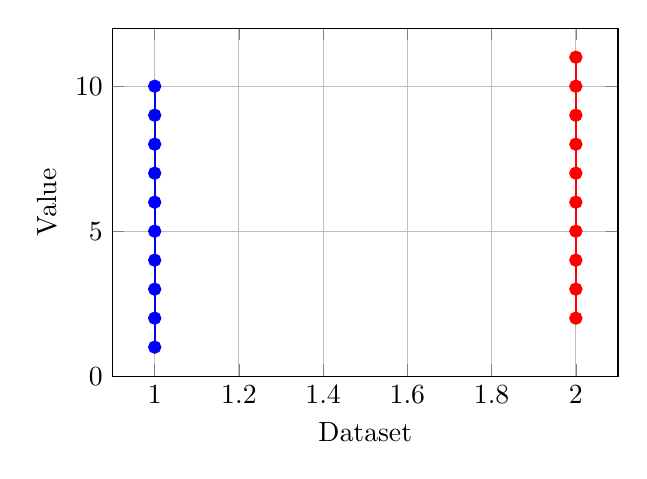
\begin{tikzpicture}
\begin{axis}[
    xlabel={Dataset},
    ylabel={Value},
    grid=both,
    width=8cm,
    height=6cm,
    ymin=0, ymax=12
]
% Simple box plot representation
\addplot[thick, blue, mark=*, mark size=2pt] coordinates {
    (1,1) (1,2) (1,3) (1,4) (1,5) (1,6) (1,7) (1,8) (1,9) (1,10)
};
\addplot[thick, red, mark=*, mark size=2pt] coordinates {
    (2,2) (2,3) (2,4) (2,5) (2,6) (2,7) (2,8) (2,9) (2,10) (2,11)
};
\end{axis}
\end{tikzpicture}
\end{center}

\footnotesize
Simplified box plot representation with scatter points
\end{frame}